\ylDisplay{Voltmeeter} % Ülesande nimi
{Tundmatu autor} % Autor
{piirkonnavoor} % Voor
{2016} % Aasta
{P 4} % Ülesande nr.
{2} % Raskustase
{
% Teema: Elektriõpetus

\ifStatement
Voltmeeter on ühendatud joonisel näidatud viisil skeemi, mis koosneb neljast ühesugusest takistist $R$ ning patareist pingega $E = 9$ $V$. Leidke voltmeetri näit.
\begin{center}
	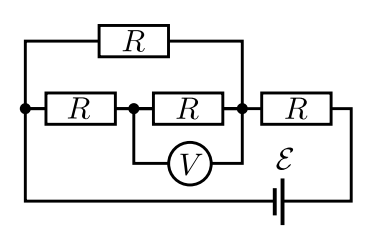
\includegraphics[width=0.5\linewidth]{2016-v2p-04-yl.png}
\end{center}
\fi



\ifHint
Leia esmalt rööpühenduse ja seejärel ahela kogutakistus ning seeläbi saad leida voolutugevuse.
\fi

\ifSolution
Rööpühendusega skeemiosa takistus on $R_r = 1/(1/R + 1/2R) = 2/3 R$ ning ahela kogutakistus $R_k = R_r + R = 5/3R$. Ahelat läbiv voolutugevus on seega $I = U/R_k = (3/5)*U/R$. Ahela rööpühendusega osale langeb pinge $U_r = I*R_r = 2/5 U$, mis on sama kummalgi rööpühenduse osal. Sellest pingest omakorda pool langeb voltmeetriga ühendatud takistile. Niisiis, $U_v = 1/2U_r = 1/5 U = 1,8$ $V$.
\fi
}
